\documentclass[11pt]{article}

\newcommand{\squishlist}{
   \begin{list}{$\bullet$}
    { \setlength{\itemsep}{0pt}      \setlength{\parsep}{3pt}
      \setlength{\topsep}{3pt}       \setlength{\partopsep}{0pt}
      \setlength{\leftmargin}{1.5em} \setlength{\labelwidth}{1em}
      \setlength{\labelsep}{0.5em} } }

\newcommand{\squishend}{
    \end{list}  }

\usepackage{times}
\usepackage{mathptm}
\usepackage{fullpage}
\usepackage{graphicx}

\begin{document}

\begin{center}
{\bf{Regis University -- Physics 305A -- Fall 2019}} \\
{\bf{Lab 3: Force Table}} \\
\medskip
\end{center}

\medskip

In this lab, you will begin to build your physical intuition about forces and 
improve your ability to calculate with vectors.

\bigskip

\begin{center}
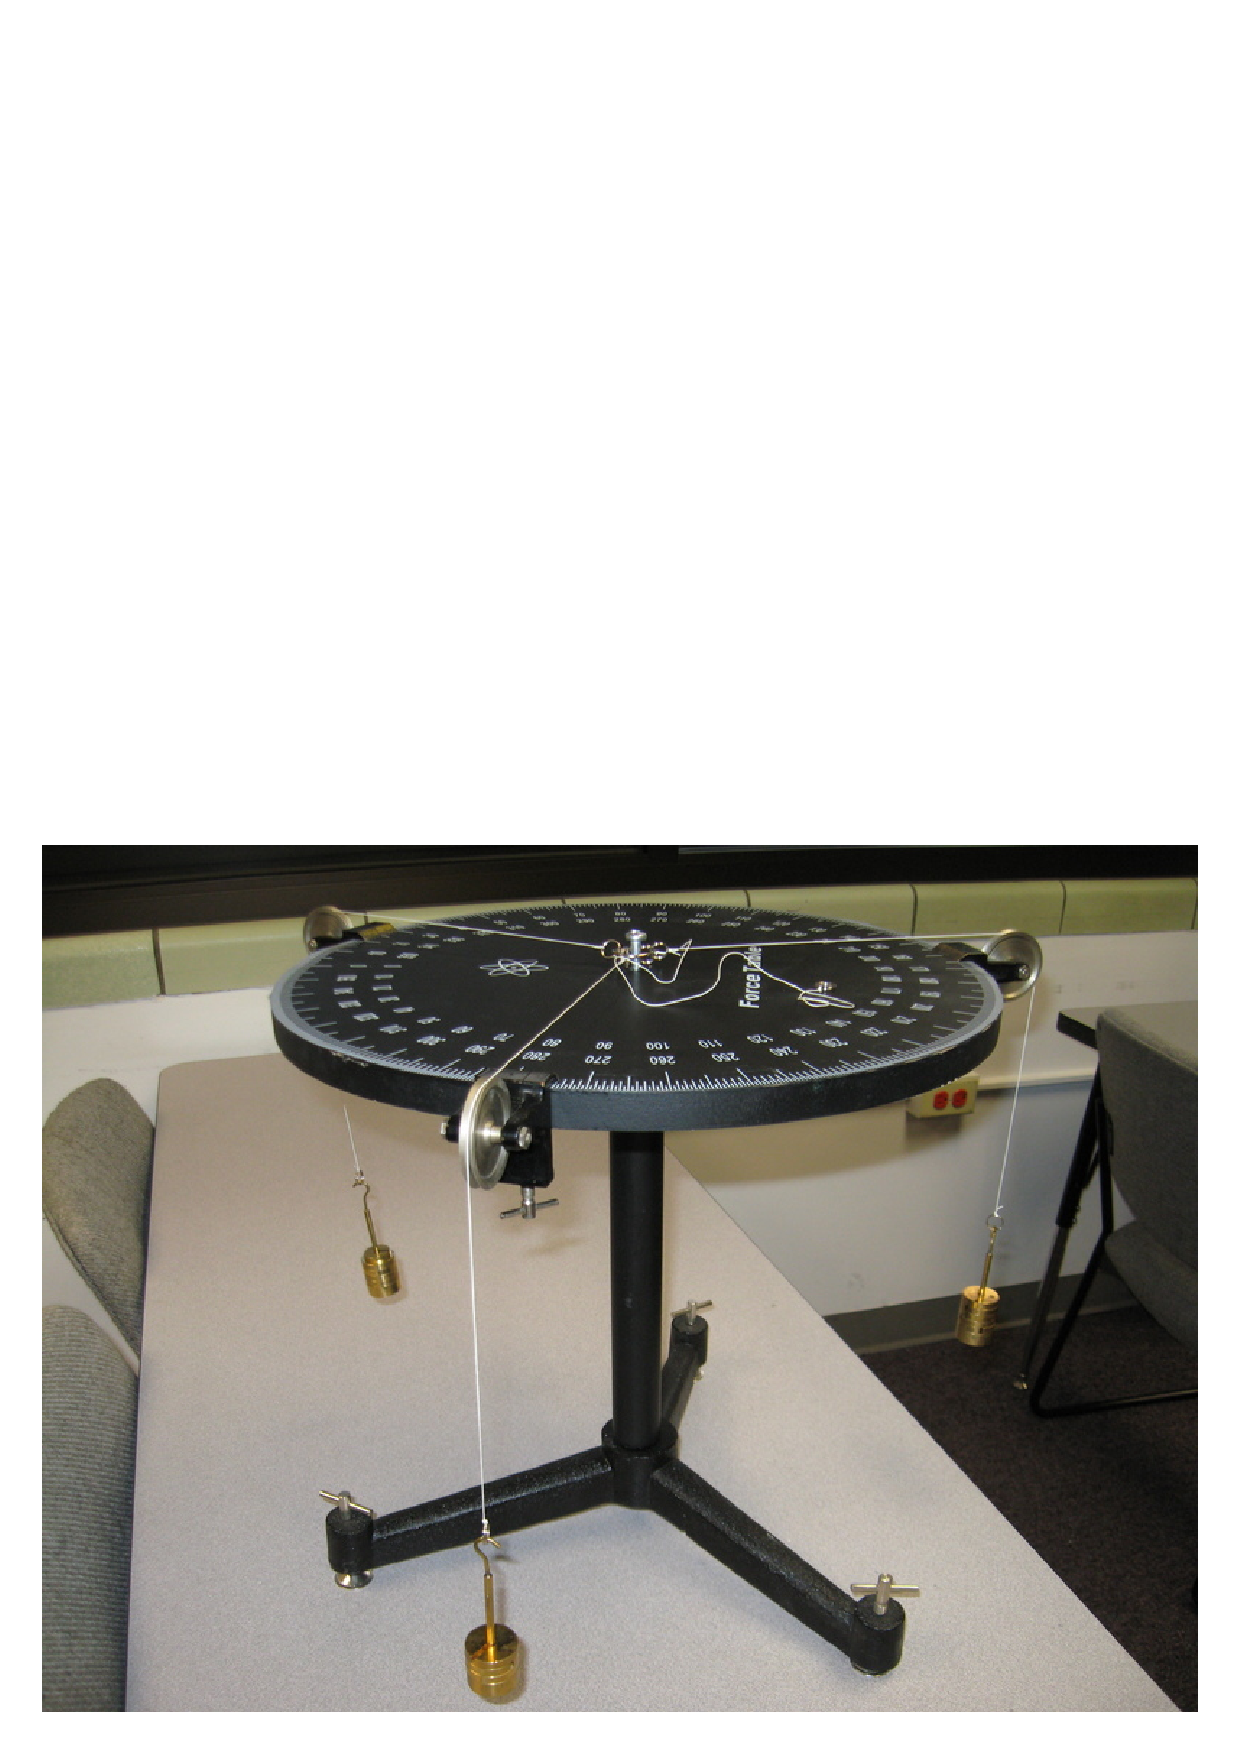
\includegraphics[height=0.30\textheight]{force_table_side1.pdf}
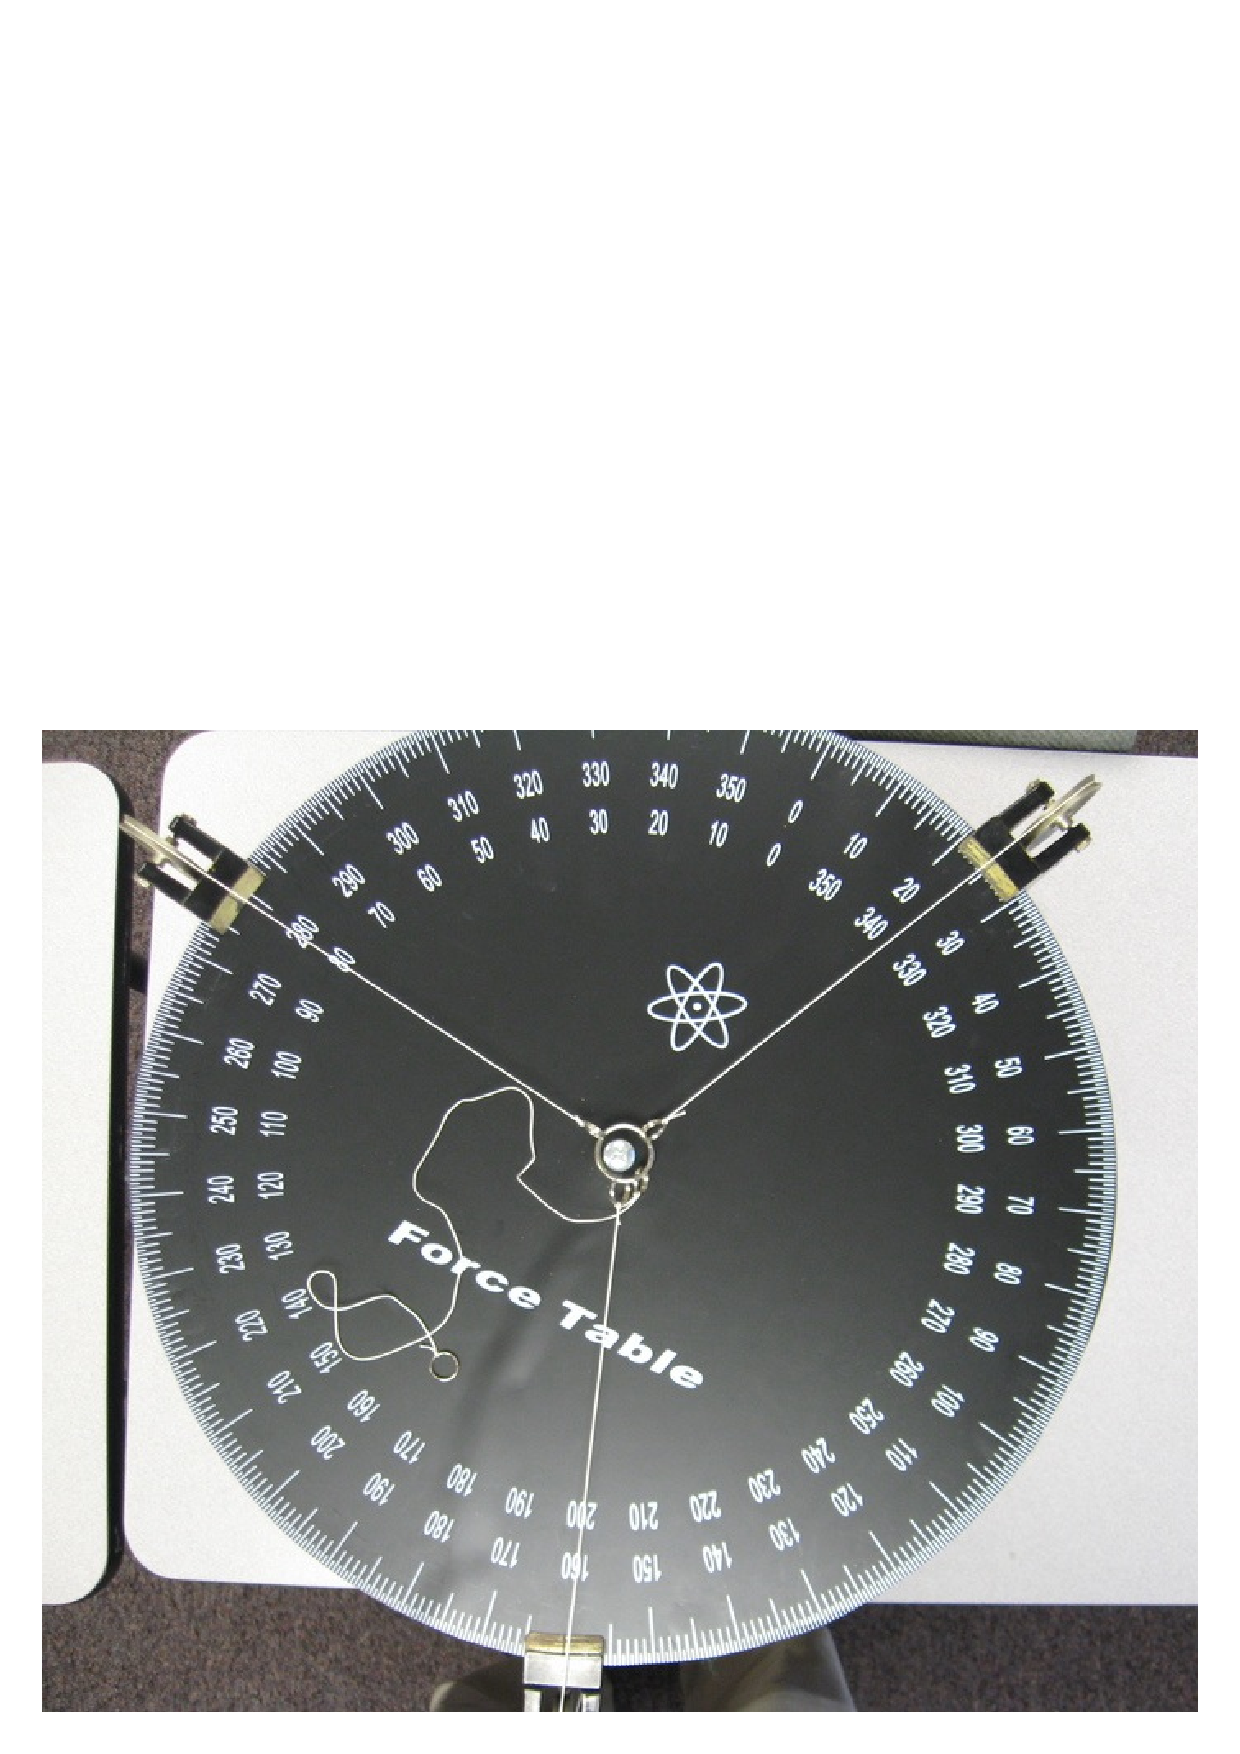
\includegraphics[height=0.30\textheight]{force_table_top1.pdf}
\end{center}

The force table is shown ``in action'' in the photographs above; we have a 
number of models that look somewhat different, but the basic principle is 
the same.  It is marked with an angular scale.  Pulleys can be clamped onto
it at any position around the circumference, allowing you to hang masses
on strings from any angle.  These strings are linked together by a ring;
your goal is to find a configuration in which the net force on the ring 
is zero (well, at least very small) so that it remains balanced, 
in static equilibrium.

The table below specifies the magnitude and direction of two forces for
various force table ``problems'':

\begin{center}
\begin{tabular}{l|ll|ll}
\hline
Problem & Force 1 & Angle 1 & Force 2 & Angle 2 \\
\hline
A & 1.22~N  & 0$^\circ$ & 1.47~N & 85$^\circ$ \\
B & 0.88~N & 75$^\circ$ & 1.76~N & 165$^\circ$ \\
C & 1.47~N & 30$^\circ$ & 1.47~N & 118$^\circ$ \\
D & 1.96~N & 0$^\circ$ & 2.16~N & 120$^\circ$ \\
\hline
\end{tabular}
\end{center}


\medskip

\noindent For each of the problems:
\begin{enumerate}
\item Compute the magnitude and direction of a third force that would 
counterbalance the given pair, giving a net force
${\vec F}_{net} = {\vec F}_1 + {\vec F}_2 + {\vec F}_3 = \vec 0$.
Remember that, to add vectors, you must break them into their Cartesian
components and add those components.
\item Determine how much mass to hang at each position 
 to create each of these three forces: two that were given, and one that
 you just calculated.
\item Set up the force table as you have calculated.  Is the system balanced
  in static equilibrium, with the ring stationary at the center of the table?  
\item If not, you should first double-check your calculations.  If they are 
  correct, then you should be able to make it balance with a small 
  adjustment to one of the forces.  How large was this adjustment,
  as a percentage of the force itself?
\end{enumerate}  

\end{document}
